\documentclass[10pt, a4paper]{article}

% --- Grundlegende Pakete ---
\usepackage[utf8]{inputenc}      % Eingabekodierung UTF-8
\usepackage[T1]{fontenc}       % Font-Kodierung
\usepackage[ngerman]{babel}    % Deutsche Spracheinstellungen & Silbentrennung
\usepackage{newtxtext}            % Verwendung einer Serifenschrift (Times-ähnlich für Zeitungslook)
\usepackage{graphicx}          % Für Bilder (Platzhalter hier)
\usepackage{geometry}          % Seitenlayout anpassen
\usepackage{multicol}          % Für mehrspaltigen Text
\usepackage{caption}           % Für Bildunterschriften
\setlength\parindent{0pt}
% --- Seitenlayout ---
\geometry{
    a4paper,
    left=15mm,
    right=15mm,
    top=7.5mm,  % Etwas weniger Rand oben, um Titel näher an Kopfzeile zu bringen
    bottom=15mm,
    %headheight=15pt,
    includehead % Kopfzeile soll Teil des oberen Randes sein
}
\setlength{\columnsep}{1cm} % Abstand zwischen den Spalten

% --- Einfache Kopfzeile (Optional) ---
\usepackage{fancyhdr}
\pagestyle{fancy}
\fancyhf{} % löscht Kopf- und Fußzeilen
\renewcommand{\headrulewidth}{0pt} % Keine Linie unter Kopfzeile
\chead{\small DIE ASHFALL GAZETTE \quad | \quad Black Creek Chronik \quad | \quad [Datum der Ausgabe, z.B. 15. Oktober 19XX]}

% --- Hilfsmakro für etwas mehr Abstand vor Überschriften ---
\newcommand{\articlesep}{\vspace{0.8em}}

% --- Dokument Beginn ---
\begin{document}
\frenchspacing % Verhindert zusätzliche Leerräume nach Satzzeichen, üblich in Zeitungen

% --- Zeitungstitel ---
\begin{center}
    \vspace*{-2em} % Kleiner Abstand zur Kopfzeile
    \Huge \textbf{DIE ASHFALL GAZETTE} \\
    \large Unabhängige Nachrichten für Black Creek und Umgebung \\
    \normalsize Ausgabe Nr. 42 \quad | \quad Mittwoch, [Datum der Ausgabe] \quad | \quad Preis: 15 Cent
\end{center}
% \vspace{-1em} % Entfernt, um Titel näher an Header zu rücken (oder reduzierten Wert nehmen)
\hrulefill % Trennlinie
% \vspace{-1em} % Entfernt

% --- Mehrspaltiger Bereich ---
\begin{multicols}{3} % Drei Spalten

% --- Titelschlagzeile ---
\large \textbf{SCHOCK IN BLACK CREEK: FAMILIENTRAGÖDIE ERSCHÜTTERT ISOLIERTE GEMEINDE} \normalsize \\
\textit{Von unserem Korrespondenten} \\

\textbf{BLACK CREEK -} Die sonst so ruhige Holzfällergemeinde Black Creek steht unter Schock, nachdem am vergangenen Dienstag der Vorarbeiter Samuel Harmon (†42) offenbar seine Frau Mary (†39) und seine beiden Kinder, Timmy (†11) und Sarah (†8), auf grausame Weise tötete, bevor er sich selbst das Leben nahm. Sheriff Brody fand die Leichen im Haus der Familie, nachdem Nachbarn Alarm geschlagen hatten.

\begin{center}
    % Bild Platzhalter - ersetze Pfad nach Bedarf
    \fbox{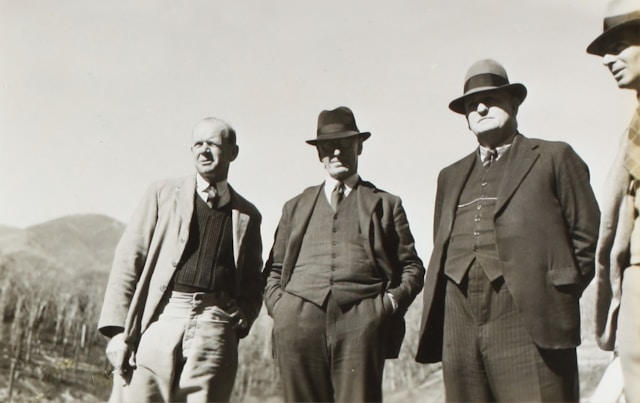
\includegraphics[width=0.9\linewidth]{museums-victoria-rcES3Cqw6z8-unsplash.jpg}}
    \captionof*{figure}{\small Sheriff Brodys Büro in Black Creek. Die Ermittlungen laufen auf Hochtouren.}
\end{center}

Die Details der Tat sind verstörend und haben die kleine Gemeinde tief erschüttert. "So etwas hat es hier noch nie gegeben", sagte ein langjähriger Bewohner, der anonym bleiben möchte. "Sam war immer ein ruhiger Kerl, stand aber unter Druck, wie wir alle hier." Die wirtschaftlich angeschlagene Stadt leidet seit Monaten unter Auftragsrückgängen im Holzgeschäft.

Sheriff Brody äußerte sich bedeckt: "Wir ermitteln in alle Richtungen, aber die Beweislage deutet auf eine schreckliche Familientragödie hin." Auf Fragen zu ungewöhnlichen Umständen am Tatort oder Gerüchten über zunehmende Spannungen in der Stadt wollte der Sheriff nicht weiter eingehen und sprach von "haltlosen Spekulationen" in einer Zeit der Trauer. Externe Ermittler wurden angefordert, um den Fall zu untersuchen.

\hrulefill % Trennlinie

% --- Weitere Artikel ---

\articlesep % Mehr Abstand
\large \textbf{Funkamateure melden Störungen} \normalsize \\
Lokale Funkamateure berichten seit Wochen über ungewöhnliche Störungen und seltsames Rauschen auf verschiedenen Frequenzen. "Es ist, als ob da etwas... mitsingt, ganz leise", beschreibt ein erfahrener Funker das Phänomen. Experten der Telekommunikationsbehörde konnten bisher keine Ursache feststellen und vermuten atmosphärische Interferenzen.

\articlesep % Mehr Abstand
\large \textbf{"Elmwood-Blues" hält an?} \normalsize \\
Berichte aus der Nachbargemeinde Elmwood deuten auf eine anhaltende Welle von Depressionen und unerklärlicher Lethargie hin. Ärzte vor Ort sind ratlos. Einige Bewohner sprechen von einem "grauen Schleier", der über dem Ort liege.

\articlesep % Mehr Abstand
\large \textbf{Streit um neues Sägewerk} \normalsize \\
Die Pläne für ein neues, modernes Sägewerk spalten die Gemeinde. Während einige auf neue Arbeitsplätze hoffen, fürchten andere Lärm und Umweltbelastung. Die Debatte wird zunehmend hitzig geführt, letzte Woche kam es beinahe zu Handgreiflichkeiten bei der Gemeinderatssitzung.

\articlesep % Mehr Abstand
\large \textbf{Jäger besorgt: Wildtiere verhalten sich seltsam} \normalsize \\
Erfahrene Jäger und Förster aus der Region berichten vermehrt über ungewöhnliches Verhalten von Wildtieren. Rehe würden reglos am Waldrand verharren, Vögel scheinen nachts zu singen, und einige Bären wirken laut Berichten ungewöhnlich apathisch oder aggressiv. Eine natürliche Ursache konnte bisher nicht identifiziert werden.

% --- Kleinanzeigen / Vermischtes ---
\hrulefill % Trennlinie

\small
\textbf{Kleinanzeigen:} Suche dringend: Alte Karten oder Aufzeichnungen über die 'Stillen Orte' in den Wäldern um Black Creek. Diskrete Bezahlung. Chiffre 1138. --- Verkaufe gebrauchten Holzspalter, Tel. 555-123. --- Benötige Hilfe bei Dachreparatur, schlechter Zustand. Biete Verpflegung. Melden bei Miller, Bachstr. 3. \\
\textbf{Kurzmeldung:} Vandalismus an Kapelle: Unbekannte beschmierten die alte Waldkapelle mit seltsamen, teerartigen Symbolen. Sheriff Brody bittet um Hinweise. \\
\textbf{Gemeinderat:} Antrag auf zusätzliche Straßenbeleuchtung abgelehnt. Mittel fehlen. \\
\textbf{Polizeibericht:} Meldungen über seltsame Lichter über den westlichen Wäldern am Wochenende eingegangen. Ursprung ungeklärt, keine weiteren Maßnahmen. \\
\normalsize
\hrulefill % Trennlinie

% --- Meinung / Leserbriefe ---
\large \textbf{Leserbriefe} \normalsize \\
"Wann tut endlich jemand was gegen die Zustände hier? Die Stimmung wird immer gereizter. Letzte Woche gab es schon wieder eine Schlägerei im 'Letzten Span'. Es liegt was in der Luft, und es riecht nicht gut..." - \textit{Besorgter Bürger} \\

\vspace{0.5em} % Kleiner Abstand
\textit{Kommentar der Redaktion: Die Tragödie der Familie Harmon muss uns allen eine Warnung sein. Der wirtschaftliche Druck und die Isolation fordern ihren Tribut. Wir müssen zusammenhalten, bevor noch Schlimmeres passiert...}

\hrulefill % Trennlinie

% --- Wissenschaft & Technik / Wetter ---
\large \textbf{Wissenschaft \& Technik} \normalsize \\
\textbf{Vortrag von Dr. Thorne abgesagt:} Der geplante Gastvortrag von Dr. Aris Thorne an der Miskatonic University über "Kosmische Zyklen und subtile Energiefluktuationen" wurde kurzfristig abgesagt. Universitätskreise sprechen von "methodischen Bedenken" gegenüber Thornes umstrittenen Theorien. Experten raten zur Vorsicht bei der Interpretation seiner Thesen. \\

\vspace{0.8em}
\large \textbf{Wettervorhersage} \normalsize \\
Überwiegend bedeckt mit gelegentlichem Nieselregen. Temperaturen bleiben ungewöhnlich kühl für die Jahreszeit. Sicht kann durch lokalen Bodennebel beeinträchtigt sein. Meteorologen warnen vor unerwarteten, lokalen Windböen in den Abendstunden. Keine Besserung in Sicht. \\

\end{multicols} % Ende des mehrspaltigen Bereichs

\end{document}